\documentclass{ximera}

\usetikzlibrary{hobby}

\title{Functions}
\begin{document}
\begin{abstract}
\end{abstract}
\maketitle

You've certainly seen many functions before. For example, you've worked with linear functions, such as
\[
f(x) = 3x+2,
\]
quadratic functions, such as
\[
h(t) = -4.9t^2 + 20t + 5,
\]
and more complicated functions such as
\[
g(x) = e^{5\sin(x^2)}+\ln \cot x.
\]
You've seen functions of more than one variable in the form of linear transformations, such as
\begin{align*}
&T:\mathbb{R}^2\rightarrow\mathbb{R}^3,\\
&T(x,y) = \left(\begin{array}{cc}
1 & 2\\
0 & -1\\
1 & 2
\end{array}\right)
\left(\begin{array}{c}
x\\
y
\end{array}\right).
\end{align*}

Not surprisingly, in multivariable calculus, we'll be studying functions of more than one variable. Before starting to work with these functions, we now cover some of the fundamental definitions and properties related to functions in general, beginning with the definition of a function.

\section*{Definition of a function}

Although we'll often think of a function as some rule, such as $f(x) = x^2$. However, a function really consists of three pieces: a domain, a codomain, and some sort of assignment. This assignment could be given by a simple rule, like $f(x) = x^2$, or could be much more difficult to describe.

\begin{definition}
For sets $X$ and $Y$, a \emph{function} $f:X\rightarrow Y$ from $X$ to $Y$ assigns an element of $Y$ to each element of $X$.

We call $X$ the \emph{domain} of $f$, and $Y$ the \emph{codomain} of $f$.
\end{definition}

You might have seen some sort of ``blob'' diagram like the one below, showing that each element of $X$ gets mapped to some element of $Y$.

\begin{image}
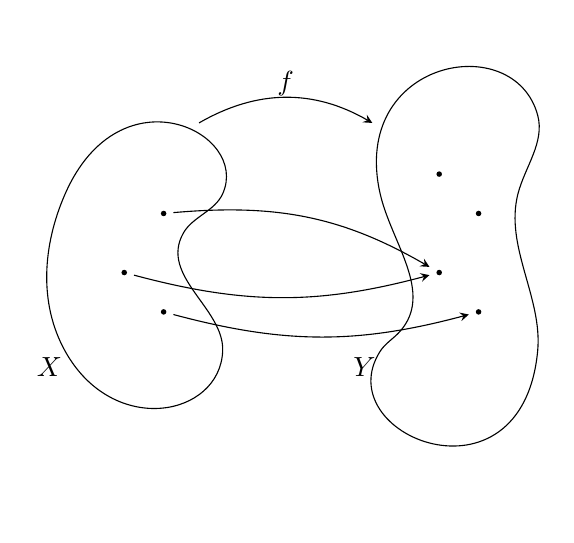
\begin{tikzpicture}
%% domain
\path[draw,use Hobby shortcut,closed=true]
(0,0) .. (0,2) .. (2,2) .. (1.5,1.5) .. (2,0);
\node at (-.2,-.2) {$X$};
%% codomain
\begin{scope}[xshift=4cm]
\node at (-.2,-.2) {$Y$};
\path[draw,use Hobby shortcut,closed=true]
(0,0) .. (.25,.25) .. (0,2) .. (2,3) .. (1.75,2) .. (2,0);
\end{scope}
%% arrow
\node at (2.8,3.4) {$f$};
\path[draw]
(1.7, 2.9) edge[out=30,in=150,-stealth] (3.9,2.9);
%% X points
\node at (1.25,.5) (x1){};
\fill (1.25,.5) circle(1pt);
\node at (.75,1) (x2){};
\fill (.75,1) circle(1pt);
\node at (1.25,1.75) (x3){};
\fill (1.25,1.75) circle(1pt);
%% Y points
\begin{scope}[xshift=4cm]
\node at (1.25,.5) (y1){};
\fill (1.25,.5) circle(1pt);
\node at (.75,1) (y2){};
\fill (.75,1) circle(1pt);
\node at (1.25,1.75) (y3){};
\fill (1.25,1.75) circle(1pt);
\node at (.75,2.25) (y4){};
\fill (.75,2.25) circle(1pt);
\end{scope}
%% arrows
\path[draw]
(x1) edge[out=-15,in=195,-stealth] (y1);
\path[draw]
(x2) edge[out=-15,in=195,-stealth] (y2);
\path[draw]
(x3) edge[out=5,in=150,-stealth] (y2);
\end{tikzpicture}
\end{image}

\begin{example}
We can define a function $f:\mathbb{R}^2\rightarrow\mathbb{R}$ by $f(x,y) = xy$.

We can define a function $g:\mathbb{R}^2\rightarrow\mathbb{R}^3$ by $g(x,y) = (x+y, x-y, xy)$.

For $U = \{(x,y,z)\neq (0,0,0)\}\in\mathbb{R}^3$, we can define a function $h:U\rightarrow \mathbb{R}^2$ by $h(x,y,z) = \left(\frac{x}{x^2+y^2+z^2}, \frac{y}{x^2+y^2+z^2}\right)$.

\end{example}


We can think of $X$ as the set of inputs to a function, and $Y$ as the set containing the outputs. Each input coming from the set $X$ has to have some corresponding output, but some elements of $Y$ might not actually occur as outputs of the function.

\begin{problem}
Which of the following are functions? Select All that apply.
\begin{selectAll}
\choice[correct]{$f:\mathbb{R}\rightarrow\mathbb{R}$ defined by $f(x) = x^2$}
\choice[correct]{$f:\mathbb{R}^2\rightarrow\mathbb{R}$ defined by $f(a,b) = a-b$}
\choice{$f:\mathbb{R}\rightarrow\mathbb{R}$ defined by $f(x) = \pm x$}
\choice[correct]{$f:\mathbb{R}\rightarrow\mathbb{R}^2$ defined by $f(x) = (x,x)$}
\end{selectAll}
\end{problem}

If we would like to refer to the elements in the codomain which actually do occur as outputs, we call this the range of $f$.

\begin{definition}
The \emph{range} of a function $f:X\rightarrow Y$ is the set of elements $y\in Y$ such that there is some $x\in X$ with $f(x) = y$. That is, there is some input $x$ that has $y$ as an output. In set notation, we write
\[
\textrm{Range }f = \{y\in Y\,:\, y = f(x) \textrm{ for some } x\in X\}.
\]
\end{definition}

We can visualize the range as a smaller set contained within the codomain.

\begin{image}
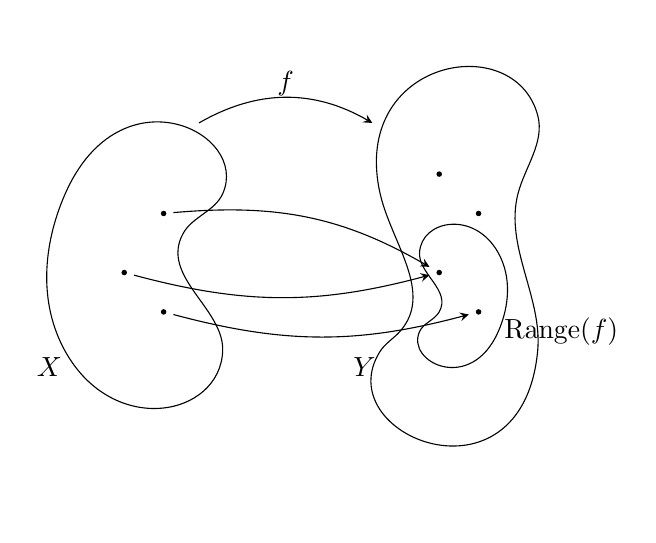
\begin{tikzpicture}
%% domain
\path[draw,use Hobby shortcut,closed=true]
(0,0) .. (0,2) .. (2,2) .. (1.5,1.5) .. (2,0);
\node at (-.2,-.2) {$X$};
%% codomain
\begin{scope}[xshift=4cm]
\node at (-.2,-.2) {$Y$};
\path[draw,use Hobby shortcut,closed=true]
(0,0) .. (.25,.25) .. (0,2) .. (2,3) .. (1.75,2) .. (2,0);
%% range
\node at (2.3,.25) {Range$(f)$};
\path[draw,use Hobby shortcut,closed=true]
(.5,.25) .. (.75,.5) .. (.5,1.25) .. (1.5,1.25) .. (1.5,.25);
\end{scope}
%% arrow
\node at (2.8,3.4) {$f$};
\path[draw]
(1.7, 2.9) edge[out=30,in=150,-stealth] (3.9,2.9);
%% X points
\node at (1.25,.5) (x1){};
\fill (1.25,.5) circle(1pt);
\node at (.75,1) (x2){};
\fill (.75,1) circle(1pt);
\node at (1.25,1.75) (x3){};
\fill (1.25,1.75) circle(1pt);
%% Y points
\begin{scope}[xshift=4cm]
\node at (1.25,.5) (y1){};
\fill (1.25,.5) circle(1pt);
\node at (.75,1) (y2){};
\fill (.75,1) circle(1pt);
\node at (1.25,1.75) (y3){};
\fill (1.25,1.75) circle(1pt);
\node at (.75,2.25) (y4){};
\fill (.75,2.25) circle(1pt);
\end{scope}
%% arrows
\path[draw]
(x1) edge[out=-15,in=195,-stealth] (y1);
\path[draw]
(x2) edge[out=-15,in=195,-stealth] (y2);
\path[draw]
(x3) edge[out=5,in=150,-stealth] (y2);
\end{tikzpicture}
\end{image}

\begin{example}
Consider the function $f:\mathbb{R}^2\rightarrow\mathbb{R}$ defined by $f(x,y) = xy$. For any real number $r$, $r = f(1,r)$, so $r$ is in the range of $f$. Thus, the range of $f$ is all real numbers, $\mathbb{R}$.

We can define a function $g:\mathbb{R}^2\rightarrow\mathbb{R}^3$ by $g(x,y) = (x+y, x-y, xy)$. In this case, the range of $g$ is the set $\{(x+y,x-y,xy)\;:\;x,y\in\mathbb{R}\}$, and it's somewhat difficult to find a simpler way to describe the range. However, we can see that the range of $g$ is not all of $\mathbb{R}^3$, since $(1,2,0)$ is not in the range of $g$. We can see this by writing $(1,2,0) = (x+y,x-y,xy)$, and trying to solve for $x$ and $y$. Here, $0=xy$ implies that we must have $x=0$ or $y=0$. If $x=0$, the first and second components give us $y=1$ and $y=-2$, a contradiction. If $y=0$, the first and second components give us $x=1$ and $x=2$, also a contradiction. Thus, $(1,2,0)$ is not in the range of $g$.
\end{example}

\begin{problem}
What is the range of the function $f:\mathbb{R}\rightarrow \mathbb{R}^2$ defined by $f(x) = (x,x)$?
\begin{multipleChoice}
\choice{$\mathbb{R}^2$}
\choice{$\mathbb{R}$}
\choice[correct]{$\{(a,b)\in\mathbb{R}^2\,:\,a=b\}$}
\choice{$\{(a,b)\in\mathbb{R}^2\,:\,a=b\}$}
\end{multipleChoice}
\end{problem}

Sometimes we work with functions that aren't defined on all of $\mathbb{R}^n$. When the domain of $f$ is a subset $D$ of $\mathbb{R}^n$, we write
\[
f:D\subset\mathbb{R}^n\rightarrow\mathbb{R}^m.
\]
When we're working with functions on subsets of $\mathbb{R}^n$, we'll frequently want to work with the largest possible set that the function is defined on. We call this the \emph{natural domain} of the function.

Often, we'll define a function just by giving a ``rule'' determining its assignment, and in this case, you should assume that the domain is the natural domain.

\begin{problem}
What is the natural domain of the function $f(x,y) = \dfrac{x}{x-y}$?
\begin{multipleChoice}
\choice{$\mathbb{R}^2$}
\choice{$\mathbb{R}^2 \setminus \{(0,0)\}$}
\choice{$\mathbb{R}^2\setminus\{(a,b)\,:\,a=0\textrm{ or }b=0\}$}
\choice[correct]{$\mathbb{R}^2\setminus\{(x,y)\,:\,a=b\}$}
\end{multipleChoice}
\end{problem}

\section*{Types of functions}

In some special situations, every element of $Y$ really does appear as an output of the function $f$. In this case, we say that $f$ is onto, or surjective.

\begin{definition}
A function $f:X\rightarrow Y$ is \emph{onto}, or \emph{surjective}, if for every element $y\in Y$, there is some $x\in X$ such that $f(x) = y$. We can also write this condition as 
\[
Y = \textrm{Range }f.
\]
\end{definition}

We can visualize this as every element of $Y$ getting mapped to by some element of $X$, and possibly more than one element.

\begin{image}
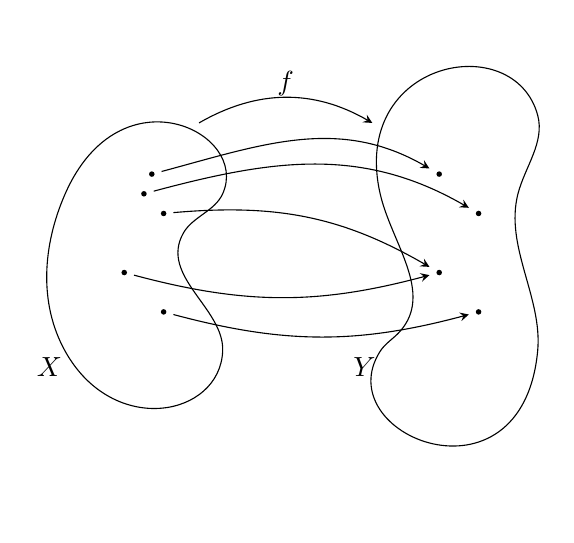
\begin{tikzpicture}
%% domain
\path[draw,use Hobby shortcut,closed=true]
(0,0) .. (0,2) .. (2,2) .. (1.5,1.5) .. (2,0);
\node at (-.2,-.2) {$X$};
%% codomain
\begin{scope}[xshift=4cm]
\node at (-.2,-.2) {$Y$};
\path[draw,use Hobby shortcut,closed=true]
(0,0) .. (.25,.25) .. (0,2) .. (2,3) .. (1.75,2) .. (2,0);
\end{scope}
%% arrow
\node at (2.8,3.4) {$f$};
\path[draw]
(1.7, 2.9) edge[out=30,in=150,-stealth] (3.9,2.9);
%% X points
\node at (1.25,.5) (x1){};
\fill (1.25,.5) circle(1pt);
\node at (.75,1) (x2){};
\fill (.75,1) circle(1pt);
\node at (1.25,1.75) (x3){};
\fill (1.25,1.75) circle(1pt);
\node at (1,2) (x4){};
\fill (1,2) circle(1pt);
\node at (1.1,2.25) (x5){};
\fill (1.1,2.25) circle(1pt);
%% Y points
\begin{scope}[xshift=4cm]
\node at (1.25,.5) (y1){};
\fill (1.25,.5) circle(1pt);
\node at (.75,1) (y2){};
\fill (.75,1) circle(1pt);
\node at (1.25,1.75) (y3){};
\fill (1.25,1.75) circle(1pt);
\node at (.75,2.25) (y4){};
\fill (.75,2.25) circle(1pt);
\end{scope}
%% arrows
\path[draw]
(x1) edge[out=-15,in=195,-stealth] (y1);
\path[draw]
(x2) edge[out=-15,in=195,-stealth] (y2);
\path[draw]
(x3) edge[out=5,in=150,-stealth] (y2);
\path[draw]
(x4) edge[out=15,in=150,-stealth] (y3);
\path[draw]
(x5) edge[out=15,in=150,-stealth] (y4);
\end{tikzpicture}
\end{image}

\begin{example}
Consider the function $f:\mathbb{R}^2\rightarrow\mathbb{R}$ defined by $f(x,y) = xy$. We previously showed that $\text{Range }f=\mathbb{R}$, so $f$ is onto.

Consider the function $g:\mathbb{R}^2\rightarrow\mathbb{R}^3$ defined by $g(x,y) = (x+y, x-y, xy)$. We previously showed that $\text{Range }g=\mathbb{R}^3$, so $g$ is not onto.
\end{example}

\begin{problem}
Which of the following functions are onto? Select all that apply.
\begin{selectAll}
\choice{$f:\mathbb{R}\rightarrow\mathbb{R}$ defined by $f(x) = x^2$}
\choice[correct]{$f:\mathbb{R}^2\rightarrow\mathbb{R}$ defined by $f(a,b) = a-b$}
\choice{$f:\mathbb{R}\rightarrow\mathbb{R}^2$ defined by $f(x) = (x,x)$}
\choice{$f:\mathbb{R}^2\rightarrow\mathbb{R}$ defined by $f(x,y) = x^2y^2$}
\end{selectAll}
\end{problem}

Another important type of function is a one-to-one, or injective, function. For a one-to-one function, different inputs always go to different outputs.

\begin{definition}
A function $f:X\rightarrow Y$ is \emph{one-to-one}, or \emph{injective}, if whenever $f(x_1) = f(x_2)$ for $x_1,x_2\in X$, then we must have $x_1 = x_2$.

Another way to say this is that whenever $x_1\neq x_2$, we have $f(x_1)\neq f(x_2)$.


\begin{image}
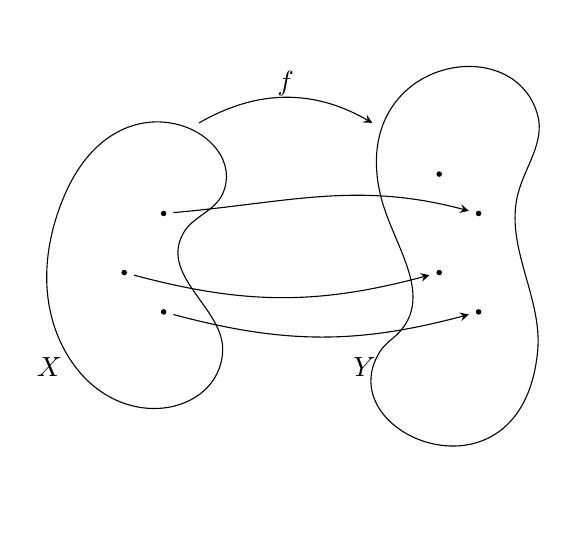
\begin{tikzpicture}
%% domain
\path[draw,use Hobby shortcut,closed=true]
(0,0) .. (0,2) .. (2,2) .. (1.5,1.5) .. (2,0);
\node at (-.2,-.2) {$X$};
%% codomain
\begin{scope}[xshift=4cm]
\node at (-.2,-.2) {$Y$};
\path[draw,use Hobby shortcut,closed=true]
(0,0) .. (.25,.25) .. (0,2) .. (2,3) .. (1.75,2) .. (2,0);
\end{scope}
%% arrow
\node at (2.8,3.4) {$f$};
\path[draw]
(1.7, 2.9) edge[out=30,in=150,-stealth] (3.9,2.9);
%% X points
\node at (1.25,.5) (x1){};
\fill (1.25,.5) circle(1pt);
\node at (.75,1) (x2){};
\fill (.75,1) circle(1pt);
\node at (1.25,1.75) (x3){};
\fill (1.25,1.75) circle(1pt);
%% Y points
\begin{scope}[xshift=4cm]
\node at (1.25,.5) (y1){};
\fill (1.25,.5) circle(1pt);
\node at (.75,1) (y2){};
\fill (.75,1) circle(1pt);
\node at (1.25,1.75) (y3){};
\fill (1.25,1.75) circle(1pt);
\node at (.75,2.25) (y4){};
\fill (.75,2.25) circle(1pt);
\end{scope}
%% arrows
\path[draw]
(x1) edge[out=-15,in=195,-stealth] (y1);
\path[draw]
(x2) edge[out=-15,in=195,-stealth] (y2);
\path[draw]
(x3) edge[out=5,in=165,-stealth] (y3);
\end{tikzpicture}
\end{image}

\end{definition}

We can visualize this as no two elements of $X$ getting mapped to the same element of $Y$.

\begin{example}
Consider the function $f:\mathbb{R}^2\rightarrow\mathbb{R}$ defined by $f(x,y) = xy$. We have that $f(0,1) = 0$ and $f(1,0)=0$, so $f$ is not one-to-one.

Consider the function $g:\mathbb{R}^2\rightarrow\mathbb{R}^3$ defined by $g(x,y) = (x+y, x-y, xy)$. We'll show that $g$ is one-to-one, by showing that if two inputs map to the same output, they must have been the same input. That is, suppose we have $g(x_1,y_1) = g(x_2,y_2)$. Then
\[
(x_1+y_1, x_1-y_1, x_1y_1) = (x_2+y_2, x_2-y_2, x_2y_2).
\]
In order to show that $x_1=x_2$ and $y_1=y_2$, we actually only need to look at the first two components, which give us the system of equations
\[
\begin{cases}
x_1+y_1 = x_2+y_2\\
x_1-y_1 = x_2-y_2\\
\end{cases}.
\]
Adding these two equations together, we obtain $2x_1 = 2x_2$, which implies $x_1 = x_2$. Substituting this into the first equation, we then also get that $y_1=y_2$. So, we have shown that $g$ is one-to-one.
\end{example}

\begin{problem}
Which of the following functions are injective? Select all that apply.
\begin{selectAll}
\choice{$f:\mathbb{R}\rightarrow\mathbb{R}$ defined by $f(x) = x^2$}
\choice{$f:\mathbb{R}^2\rightarrow\mathbb{R}$ defined by $f(a,b) = a-b$}
\choice[correct]{$f:\mathbb{R}\rightarrow\mathbb{R}^2$ defined by $f(x) = (x,x)$}
\choice{$f:\mathbb{R}^2\rightarrow\mathbb{R}$ defined by $f(x,y) = x^2y^2$}
\end{selectAll}
\end{problem}

\section*{Component functions}

When we're trying to understand the behavior of a function $f:X\subset \mathbb{R}^n\rightarrow \mathbb{R}^m$, it can sometimes be helpful to split $\mathbb{R}^m$ into its components. From this, we get the component functions of $f$.

\begin{definition}
Let $f:X\subset \mathbb{R}^n\rightarrow \mathbb{R}^m$ be a function. The \emph{component functions} of $f$ are scalar-valued functions $f_i:X\subset\mathbb{R}^n\rightarrow\mathbb{R}$ for $1\leq i\leq m$ such that 
\[
f(\vec{x}) = (f_1(\vec{x}),f_2(\vec{x}),...,f_m(\vec{x})).
\]
\end{definition}

\begin{example}
Consider the function $g:\mathbb{R}^2\rightarrow\mathbb{R}^3$ defined by $g(x,y) = (x+y, x-y, xy)$. The component functions of $g$ are
\begin{align*}
g_1(x,y) &= x+y,\\
g_2(x,y) &= x-y,\\
g_3(x,y) &= xy.
\end{align*}
Notice that each of these is a function $\mathbb{R}^2\rightarrow\mathbb{R}$.
\end{example}

\end{document}